\documentclass[a5paper,9pt,twoside=false]{extbook}

\usepackage[ngerman]{babel}
\usepackage[utf8]{inputenc}
\usepackage[T1]{fontenc}
\usepackage[10pt]{moresize}
\usepackage[top=1.5cm, left=1.5cm, right=1.5cm, bottom=1.5cm]{geometry}
\usepackage{enumitem}
\usepackage{tabularx}
\usepackage{graphicx}
\usepackage{wrapfig}

\usepackage[babel,german=quotes]{csquotes}
\MakeOuterQuote{"}

\usepackage[sfdefault,light]{merriweather}   

\pagestyle{empty}

\title{Moby Dick in 30 Minuten}   
\author{Kathrin Passig \& Esther Seyffarth} 
\date{6. Mai 2019} 

\begin{document}


%=========================================
\begin{titlepage}

\vspace{3em}
		\centering{
			{\fontsize{40}{48}\selectfont 
			Moby Dick in 30 Minuten}
		}\\
			
		\vspace{10mm}
		\centering{\huge{Kathrin Passig \& Esther Seyffarth}}\\
		
		\vspace{1.5cm}
	
%%%%%%%%%%%%%%%%%%%%%%%%%%%%%%%%%%%%%%%%		
		
\begin{figure}[h]       
{ \centering
% Visualisierung des Plots von Moby Dick, erzeugt mithilfe von https://editor.method.ac/	
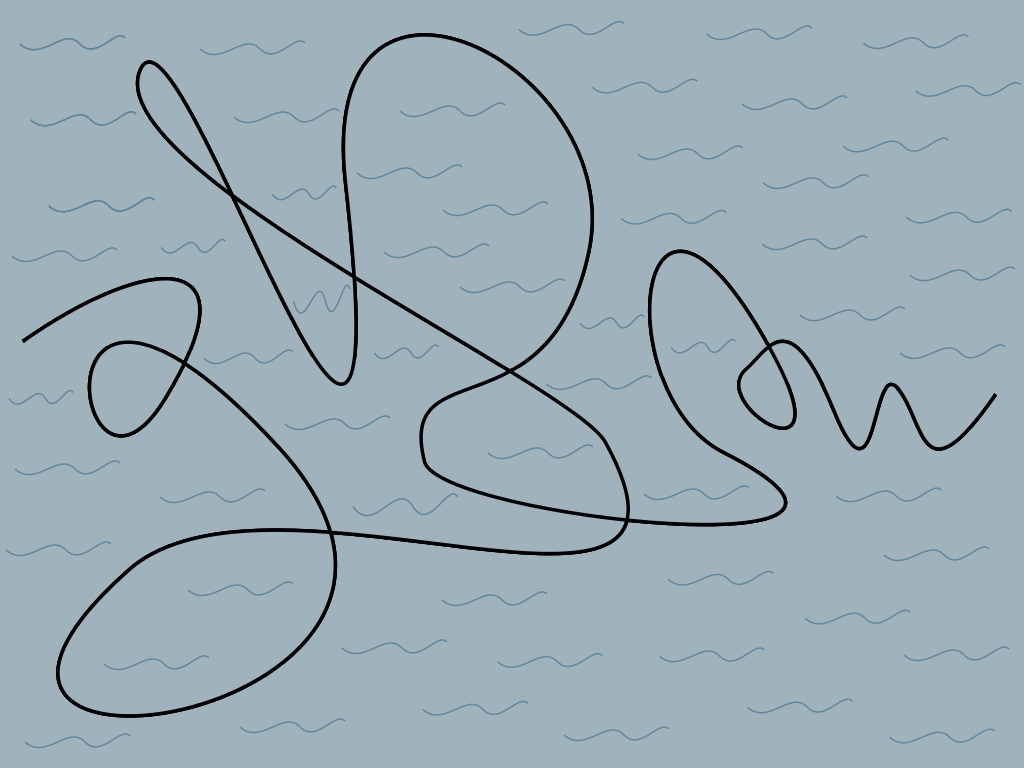
\includegraphics[width=\textwidth]{plot_curve_water.png} \\
}

\end{figure}
		
		\vspace{\fill}
		\centering \large{6. Mai 2019 // re:publica \\11:30 -- 12:00, Reader's Corner (Main Hall)}
\end{titlepage}

%=========================================

\newpage

\section*{Worum geht es in \textit{Moby Dick}?}\label{interpretationen}

\subsection*{Walfang}
\textit{Moby Dick} ist ein 1851 erschienener Roman von Herman Melville, in dem es hauptsächlich um die Walfangindustrie der damaligen Zeit geht. Zusammen mit dem Protagonisten \textbf{Ishmael} lernen wir alles, was man über Wale, Tran, Boote, Seile, Harpunen und Segel wissen muss.

\medskip

\subsection*{Rache}
\textit{Moby Dick} ist ein 1851 erschienener Roman von Herman Melville, in dem es hauptsächlich um Rache geht. \textbf{Ahab}, der Kapitän des Walfangschiffes \textit{Pequod}, wurde vom Wal \textbf{Moby Dick} verletzt und macht sich auf den Weg, den Wal zu finden, um sich an ihm zu rächen.

\medskip

\subsection*{Religion}
\textit{Moby Dick} ist ein 1851 erschienener Roman von Herman Melville, in dem es hauptsächlich um Religion geht. \textbf{Ahab}, der Kapitän des Walfangschiffes \textit{Pequod}, hat andere Ansichten als sein frommer Steuermann \textbf{Starbuck}; die beiden geraten auf einer langen Schiffsreise in zahlreiche Wortgefechte.

\medskip

\subsection*{Pokémon}
\textit{Moby Dick} ist ein 1851 erschienener Roman von Herman Melville, in dem es hauptsächlich um Pokémon geht. Die Crew des Walfangschiffs \textit{Pequod} reist mit Engelsgeduld durch die Meere der Welt und hofft, ein shiny Wailmer zu finden. Das Wailmer taucht zum Schluss zwar auf, lässt sich aber nicht fangen. \textbf{Ahab} benutzt eine Harpune, aber es ist nicht sehr effektiv. 

\medskip

\subsection*{Blockchain}
\textit{Moby Dick} ist ein 1851 erschienener Roman von Herman Melville, in dem es hauptsächlich um die Blockchain geht. Die Crew des Walfangschiffs \textit{Pequod} hofft auf großen Gewinn und investiert enorme Zeit und Ressourcen. Aber die Schwierigkeit der Aufgabe ist zu groß und die spezialisierte Hardware versagt.

\medskip

\subsection*{Feminismus}
\textit{Moby Dick} ist ein 1851 erschienener Roman von Herman Melville, in dem es hauptsächlich um Feminismus geht. Die Crew des Walfangschiffs \textit{Pequod} besteht ausschließlich aus Männern, deren toxische Vorstellung von Maskulinität letztlich ihr Untergang ist.

%%%%%%%%%%%%%%%%%%%%%%%%%%%%%%%%%%%%%%%%

\newpage
\section*{Verschiedene Vorstellungen von Walen}\label{walmalen}
\vspace{-15pt}

\begin{figure}[h]
{ \centering
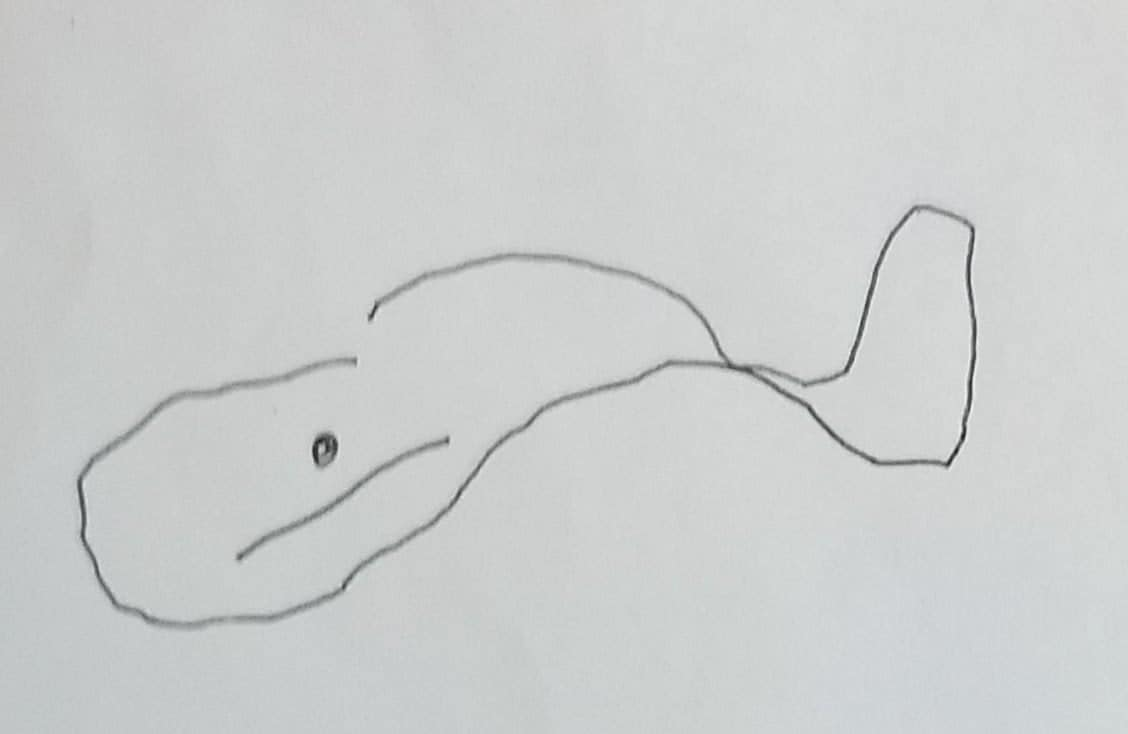
\includegraphics[width=0.6\textwidth]{kathrins_wal.jpg} \\
} \caption{Kathrins Vorstellung von einem Wal.}
\end{figure}

\noindent Bis dato ist der Pottwal aber in keinem Werke, ob wissenschaftlicher oder poetischer Natur, wirklich und vollständig mit Leben erfüllt worden. Seine Lebensgeschichte muss noch geschrieben werden, anders als die aller sonstigen gejagten Wale.

Nun bedürfen die verschiedenen Arten von Walen einer irgendwie gearteten, allgemeinverständlichen Klassifizierung, und sei sie zunächst nur ein flüchtiger Umriss, dessen einzelne Teile später von fleißigen Forschern ausgefüllt werden mögen. Da kein Besserer hervortritt, die Sache in die Hand zu nehmen, biete ich hiermit meine bescheidenen Dienste an. Ich verspreche nichts Vollkommenes, weil jedwedes Menschending, das nach Vollkommenheit strebt, just aus diesem Grunde unfehlbar fehlerhaft sein muss. Ich werde mich nicht an einer bis in alle Einzelheiten exakten Anatomie der verschiedenen Arten versuchen, noch auch nur an einer hinreichenden Beschreibung, zumindest nicht jetzt und hier.

\medskip

\noindent\footnotesize{\textit{Kapitel 32 (Cetologie)}}

\normalsize

\begin{figure}[h]
{ \centering
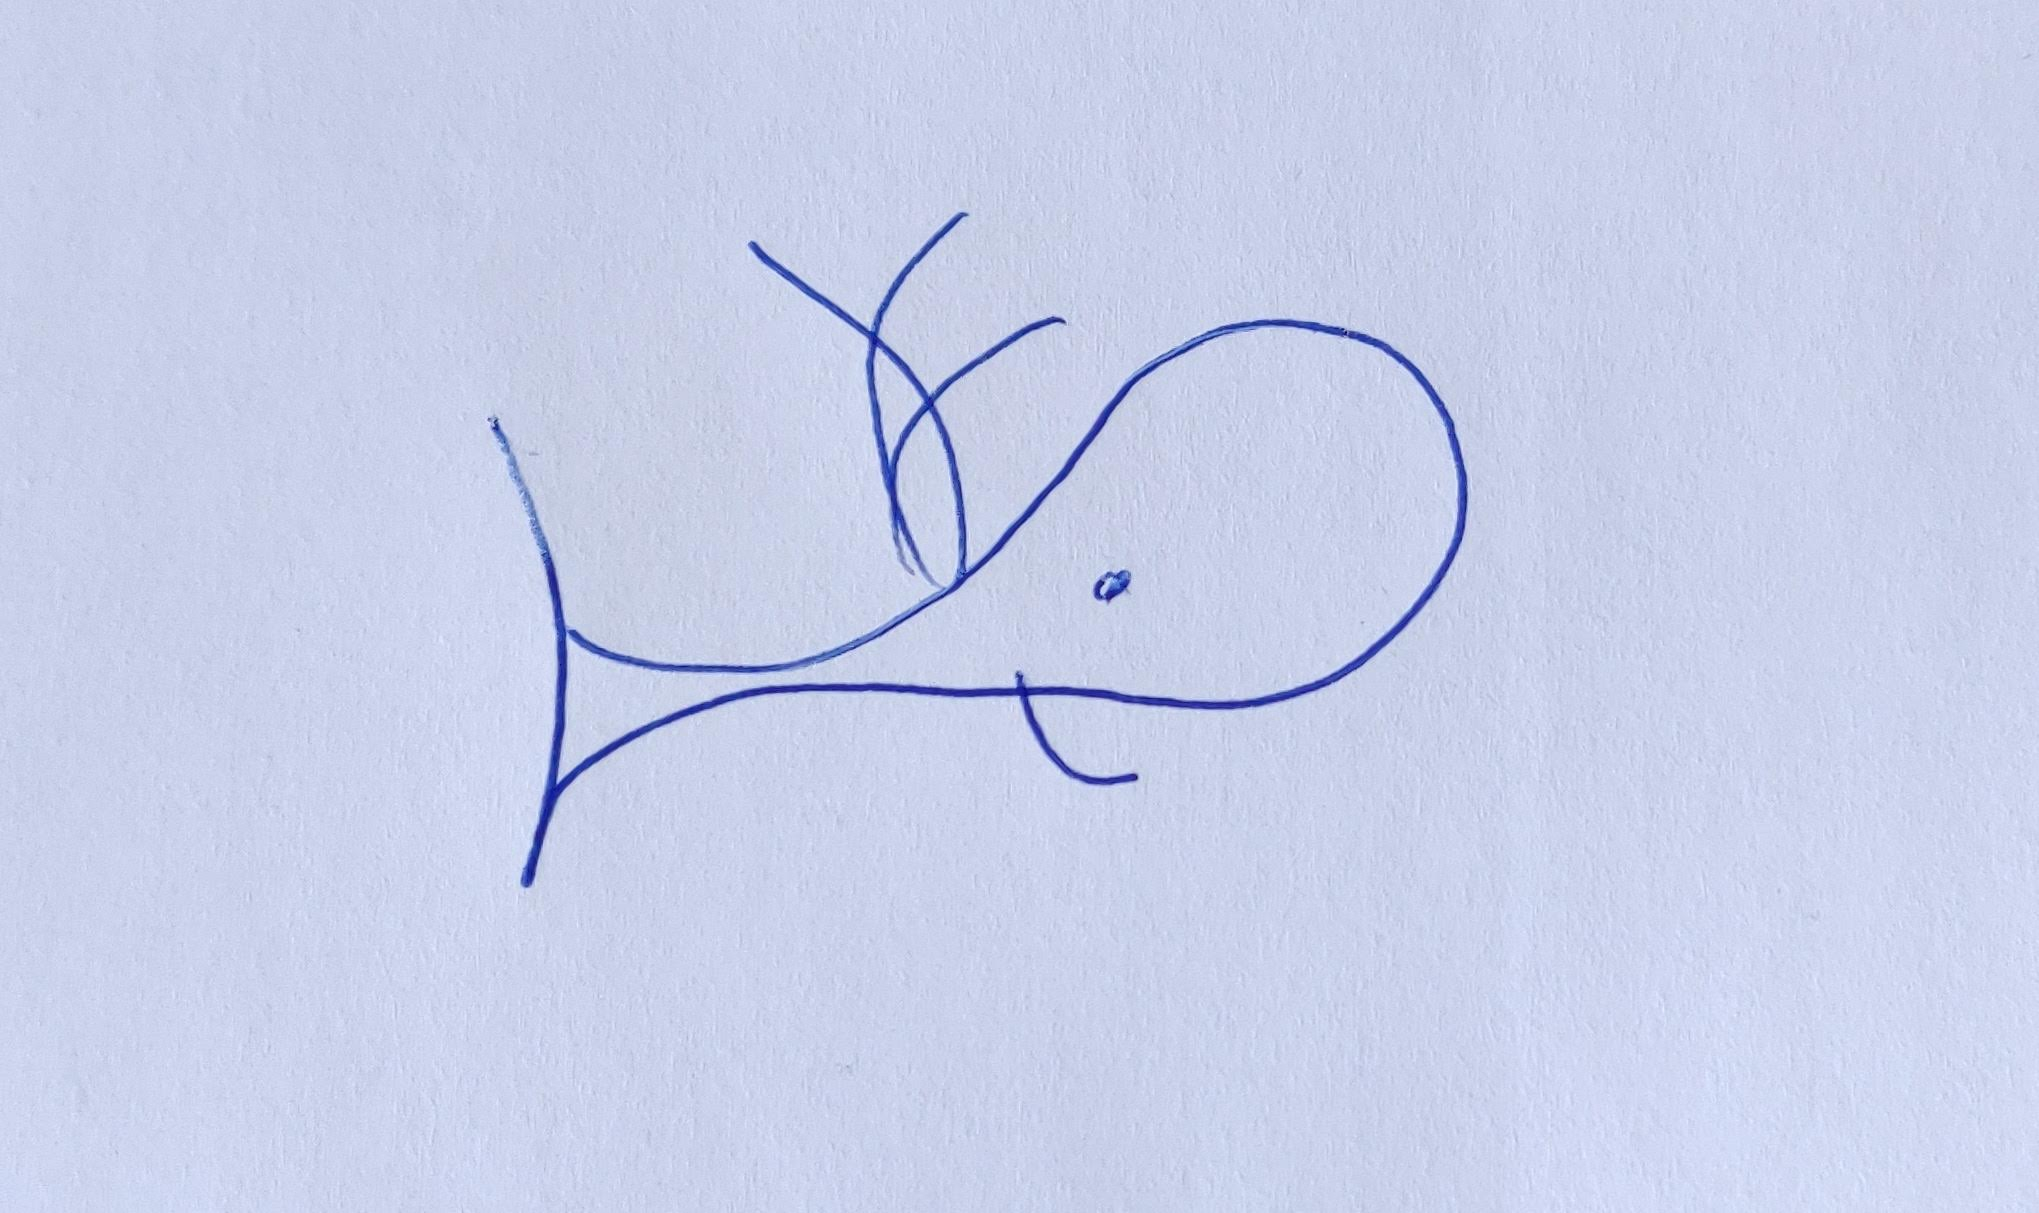
\includegraphics[width=0.6\textwidth]{esthers_wal.jpg} \\
} \caption{Esthers Vorstellung von einem Wal.}
\end{figure}

%%%%%%%%%%%%%%%%%%%%%%%%%%%%%%%%%%%%%%%%

\newpage
\section*{Kapitel, in denen nichts Wesentliches passiert}\label{irrelevantes}
\textit{Moby Dick} ist ein 1851 erschienener Roman von Herman Melville, dessen Plot oft von irrelevanten Nebensächlichkeiten unterbrochen wird. In den folgenden Kapiteln passiert z.B. überhaupt nichts Wesentliches:
\footnotesize

\bigskip

\noindent
{\renewcommand{\arraystretch}{1.6} % etwas erhöhter Zeilenabstand
\begin{tabularx}{\textwidth}{X|X|X}
  \textbf{1} Schemen & \textbf{44} Die Seekarte & \textbf{80} Die Nuss\\ \hline 
  \textbf{6} Die Straße & \textbf{45} Eidesstattliche Erklärung & \textbf{82} Ruhm und Ehre des Walfangs \\ \hline 
    \textbf{7} Die Kirche & \textbf{46} Mutmaßungen & \textbf{83} Jona, historisch-kritisch betrachtet \\ \hline 
    \textbf{8} Die Kanzel & \textbf{49} Die Hyäne & \textbf{85} Der Springbrunnen \\ \hline 
    \textbf{9} Die Predigt & \textbf{53} Das Gam & \textbf{86} Der Schwanz \\ \hline 
    \textbf{14} Nantucket & \textbf{54} Die Geschichte der \textit{Town-Ho} & \textbf{88} Schulen \& Schulmeister \\ \hline 
    \textbf{15} Chowder & \textbf{55} Ungeheuerliche Zerrbilder von Walen & \textbf{89} Festfisch und Losfisch \\ \hline 
    \textbf{17} Der Ramadan & \textbf{56} Weniger fehlerhafte Bilder von Walen & \textbf{90} Kopf oder Schwanz \\ \hline 
    \textbf{20} Reger Betrieb & \textbf{57} Über Wale aus Farbe, aus Zahn \& c. & \textbf{92} Amber \\ \hline 
    \textbf{21} Es geht an Bord & \textbf{58} Krill & \textbf{94} Ein Händedruck \\ \hline 
    \textbf{22} Fröhliche Weihnachten & \textbf{60} Die Leine & \textbf{95} Der Überzieher \\ \hline 
    \textbf{23} Land in Lee & \textbf{62} Der Anwurf & \textbf{96} Die Tranöfen \\ \hline 
    \textbf{24} Der Anwalt & \textbf{63} Die Gabel & \textbf{97} Die Lampe \\ \hline 
    \textbf{25} Postskriptum & \textbf{65} Der Wal als Speisefisch & \textbf{98} Verstauen \& Aufklaren \\ \hline 
    \textbf{29} Auftritt Ahab; zu ihm, Stubb & \textbf{66} Das Haifischgemetzel & \textbf{101} Die Karaffe \\ \hline 
    \textbf{30} Die Tobackspfeife & \textbf{67} Flensen & \textbf{102} Eine Laube auf den Arsakiden \\ \hline 
    \textbf{31} Mab, die Feenkönigin & \textbf{68} Die Decke & \textbf{103} Vermessung des Walskeletts \\ \hline 
    \textbf{32} Cetologie & \textbf{69} Die Bestattung & \textbf{104} Der Wal als Fossil \\ \hline 
    \textbf{33} Der Specksijnder & \textbf{71} Die \textit{Pequod} begegnet der \textit{Jeroboam} -- Ihre Geschichte & \textbf{105} Wird der Wal kleiner? \\ \hline 
    \textbf{34} An der Kajütstafel & \textbf{74} Des Pottwals Kopf & \textbf{107} Der Zimmermann \\ \hline 
    \textbf{35} Im Masttopp & \textbf{75} Des Glattwals Kopf & \textbf{112} Der Schmied \\ \hline 
    \textbf{40} Auf der Back -- Mitternacht & \textbf{76} Der Rammbock & \textbf{114} Der Vergulder \\ \hline 
    \textbf{42} Das Weiß des Wals & \textbf{77} Das große Fass zu Heidelburgh & \textbf{116} Der sterbende Wal \\ \hline 
    \textbf{43} Horch! & \textbf{79} Die Prärie & \textbf{122} Mitternacht, oben im Rigg
\end{tabularx}
}
\normalsize

%%%%%%%%%%%%%%%%%%%%%%%%%%%%%%%%%%%%%%%%

\newpage
\section*{Kapitel, in denen Wesentliches passiert}\label{relevantes}
\textit{Moby Dick} ist ein 1851 erschienener Roman von Herman Melville, in dem die Reise eines Walfangschiffs beschrieben wird, dessen Ziel es ist, einen weißen Wal namens \textbf{Moby Dick} zu finden und zu töten. Grund dafür ist eine Auseinandersetzung, die Kapitän \textbf{Ahab} mit Moby Dick hatte. Der Plot der Geschichte spielt sich hauptsächlich in den folgenden Kapiteln ab:
\footnotesize

\bigskip

\noindent
{\renewcommand{\arraystretch}{1.6}
\begin{tabularx}{\textwidth}{X|X|X}
    \textbf{2} Die Reisetasche & \textbf{50} Ahabs Boot und Mannschaft. Fedallah & \textbf{111} Der Stille Ozean \\\hline%[6pt] 
    \textbf{3} Das Gasthaus "Zum Walfänger" & \textbf{51} Der Geisterspaut & \textbf{113} Die Esse \\ \hline 
    \textbf{4} Die Steppdecke & \textbf{52} Die \textit{Pequod} begegnet der \textit{Albatros} & \textbf{115} Die \textit{Pequod} begegnet der \textit{Bachelor} \\ \hline 
    \textbf{5} Frühstück & \textbf{59} Kalmare & \textbf{117} Die Walwache \\ \hline 
    \textbf{10} Ein Busenfreund & \textbf{61} Stubb tötet einen Wal & \textbf{118} Der Quadrant \\ \hline 
    \textbf{11} Schlafrock & \textbf{64} Stubbs Mahl & \textbf{119} Die Kerzen \\ \hline 
    \textbf{12} Biographisches & \textbf{70} Die Sphinx & \textbf{120} An Deck \\ \hline 
    \textbf{13} Schubkarren & \textbf{72} Der Affentamp & \textbf{121} Mitternacht, auf der Back \\ \hline 
    \textbf{16} Das Schiff & \textbf{73} Stubb \& Flask töten einen Glattwal & \textbf{123} Die Muskete \\ \hline 
    \textbf{18} Sein Zeichen & \textbf{78} Brunnen und Eimer & \textbf{124} Die Nadel \\ \hline 
    \textbf{19} Der Prophet & \textbf{81} Die \textit{Pequod} begegnet der \textit{Jungfrau} & \textbf{125} Log und Leine \\ \hline 
    \textbf{26} Ritter und Knappen & \textbf{84} Koppheisterwurf & \textbf{126} Die Rettungsboje \\ \hline 
    \textbf{27} Ritter und Knappen & \textbf{87} Die Große Armada & \textbf{127} Ahab und der Zimmermann \\ \hline 
    \textbf{28} Ahab & \textbf{91} Die \textit{Pequod} begegnet der \textit{Rosenknospe} & \textbf{128} Die \textit{Pequod} begegnet der \textit{Rachel} \\ \hline 
    \textbf{36} Das Achterdeck -- Ahab und alle & \textbf{93} Der Verstoßene & \textbf{129} In der Kajüte -- Ahab und Pip \\ \hline 
    \textbf{37} Sonnenuntergang & \textbf{99} Die Dublone & \textbf{130} Der Hut \\ \hline 
    \textbf{38} Dämmerung & \textbf{100} Die Pequod begegnet der \textit{Samuel Enderby} aus London & \textbf{131} Die \textit{Pequod} begegnet der \textit{Delight} \\ \hline 
    \textbf{39} Erste Nachtwache & \textbf{106} Ahabs Bein & \textbf{132} Die Symphonie \\ \hline 
    \textbf{41} Moby Dick & \textbf{108} An Deck -- Ahab und der Zimmermann & \textbf{133} Die Jagd -- Der erste Tag \\ \hline 
    \textbf{47} Der Mattenweber & \textbf{109} In der Kajüte -- Ahab und Starbuck & \textbf{134} Die Jagd -- Der zweite Tag \\ \hline 
    \textbf{48} Erstmals in den Booten & \textbf{110} Queequeg in seinem Sarg & \textbf{135} Die Jagd -- Der dritte Tag
 \end{tabularx}
 }
\normalsize

%%%%%%%%%%%%%%%%%%%%%%%%%%%%%%%%%%%%%%%%

\newpage
\section*{Moby Dick, as fast as possible}\label{textstellen}

\noindent Aus diesen Gründen also war mir die Walfangreise willkommen; die großen Schleusentore der Wunderwelt schwangen auf, und inmitten der wilden Hirngespinste, welche mich zu meinem Vorhaben drängten, trieben sie in meine innerste Seele, Paar für Paar, eine endlose Prozession von Walen, und, mitten unter ihnen, ein grandioses, verhüllendes Phantom, gleich einem Schneeberg in den Lüften.

\medskip
\noindent\footnotesize{\textit{Kapitel 1 (Schemen)}}
\normalsize

\medskip
{\centering \small*** \\}
\bigskip

\noindent Die ganze grimmige Erscheinung Ahabs und das fahle Mal, das sie zeichnete, setzten mir so stark zu, dass ich im ersten Augenblick kaum bemerkte, wieviel von diesem alles beherrschenden Ingrimm sich dem barbarischen weißen Beine verdankte, auf dem er zur Hälfte stand. Mir war schon zu Ohren gekommen, dass dieses walbeinerne Bein auf See aus dem polierten Kieferknochen des Pottwals geschnitzt worden war.

\medskip
\noindent\footnotesize{\textit{Kapitel 28 (Ahab)}}
\normalsize

\medskip
{\centering \small*** \\}
\bigskip

\noindent "Wer von euch mir einen weißköpfigen Wal mit runzliger Stirn und schiefem Maule sichtet, der drei Löcher in seiner Steuerbordfluke trägt -- hört gut zu, meine Jungs: Wer von euch mir diesen weißen Wal sichtet, der soll diese Unze Gold bekommen!"

\medskip
\noindent\footnotesize{\textit{Kapitel 36 (Das Achterdeck), Ahab zur Crew}}
\normalsize

\medskip
{\centering \small*** \\}
\bigskip

\noindent Weit über den Bug hinausgebeugt, bohrte Stubb gemächlich seine lange scharfe Lanze in den Fisch und ließ sie dort stecken, wobei er achtsam weiter bohrte und bohrte, so als suche er sorgfältig nach einer goldenen Uhr, die der Wal verschluckt haben könnte, und fürchte, sie zu zerbrechen, bevor er sie herausfischen könne.

\medskip
\noindent\footnotesize{\textit{Kapitel 61 (Stubb tötet einen Wal)}}
\normalsize

\medskip
{\centering \small*** \\}
\bigskip

\noindent Wäre nun Tashtego in diesem Haupte zu Tode gekommen, wär's wahrlich ein erlesener Tod gewesen: erstickt im weißesten und feinsten, wohlriechenden Walrat; eingesargt, aufgebahrt und bestattet in der Geheimkammer tief im Wale, in seinem Sanctum Sanctorum.

\medskip
\noindent\footnotesize{\textit{Kapitel 78 (Brunnen und Eimer)}}
\normalsize

\medskip
{\centering \small*** \\}
\bigskip

\noindent Doch wie dem auch sei, ob nun der unsichtbare, ungreifbare Geisterrat der Lüfte oder die rachsüchtigen Fürsten und Machthaber des Feuers etwas mit dem irdischen Ahab zu tun haben oder nicht, was sein Bein anging, handelte er ganz praktisch -- er rief den Zimmermann.

\medskip
\noindent\footnotesize{\textit{Kapitel 106 (Ahabs Bein)}}
\normalsize

\medskip
{\centering \small*** \\}
\bigskip

\noindent Als daraufhin manche ihrer freudigen Überraschung Ausdruck verliehen, sagte er sinngemäß, dass die Ursache seiner plötzlichen Genesung folgende sei: Als es heikel wurde, habe er sich einer Kleinigkeit an Land besonnen, welche er nicht erledigt habe, und deshalb seine Meinung geändert, was das Sterben anging -- er könne jetzt noch nicht sterben, verkündete er. %Nun aber, da er doch offensichtlich alle Vorbereitungen für seinen Tod getroffen hatte; nun, da sein Sarg erwiesenermaßen passte, kam Queequeg auf einmal wieder zu Kräften, und bald wurde die Kiste des Zimmermanns nicht mehr gebraucht.

\medskip
\noindent\footnotesize{\textit{Kapitel 110 (Queequeg in seinem Sarg)}}
\normalsize

% \medskip
% {
% \centering \small*** \\
% }
% \bigskip
% \noindent "Auch ich will, dass du mir eine Harpune machst, eine, die auch tausend Teufelsgespanne nicht zerreißen können, Perth; etwas, was im Wale steckenbleibt wie der Knochen seiner Flosse."

% \medskip
% \noindent\footnotesize{\textit{Kapitel 113 (Die Esse), Ahab zum Schmied}}
% \normalsize

\medskip
{\centering \small*** \\}
\bigskip

\noindent Wie der Arm eines Trunkenen schlug die Muskete, die immer noch auf Ahab gerichtet war, gegen das Türholz. Es war, als würde Starbuck mit einem Engel ringen. Dann aber wandte er sich ab, stellte das Todesrohr wieder in seinen Halter und ging zurück an Deck.

\medskip
\noindent\footnotesize{\textit{Kapitel 123 (Die Muskete)}}
\normalsize

\medskip
{\centering \small*** \\}
\bigskip

\noindent Freude und Kummer, Hoffnung und Furcht, alles schien vorerst im schweren Mörser von Ahabs Eisenseele zu feinstem Staub zermahlen.

\medskip
\noindent\footnotesize{\textit{Kapitel 130 (Der Hut)}}
\normalsize

\medskip
{\centering \small*** \\}
\bigskip

\noindent Sein ganzer Anblick verhieß Rache, rasche Vergeltung und ewige Arglist, und keine Macht auf Erden konnte ihn hindern, mit dem massigen weißen Klotz seiner Stirn den Bug steuerbords zu rammen, dass Masten und Männer wankten. Manche schlugen der Länge nach hin. Wie lose Flaggenknöpfe wackelten den Harpunieren droben im Rigg die Köpfe auf ihren Stiernacken. Drunten hörte man die See durch das Leck ins Schiff strömen, wie ein reißender Wildbach durch eine Bergklamm rauscht.

\medskip
\noindent\footnotesize{\textit{Kapitel 135 (Die Jagd -- Der dritte Tag)}}
\normalsize

\medskip
{\centering \small*** \\}
\bigskip

\noindent Nun flogen kleine Vögel kreischend über dem noch gähnenden Abgrund; mürrische weiße Wellen schlugen gegen seine steilen Wände; dann brach alles ein, und das große Leichentuch des Meeres wogte weiter wie vor fünf Jahrtausenden.

\medskip
\noindent\footnotesize{\textit{Kapitel 135 (Die Jagd -- Der dritte Tag)}}

\normalsize

%%%%%%%%%%%%%%%%%%%%%%%%%%%%%%%%%%%%%%%%

\newpage

\section*{Die Performerinnen}\label{aboutus}

\begin{figure}[h]
{ \centering
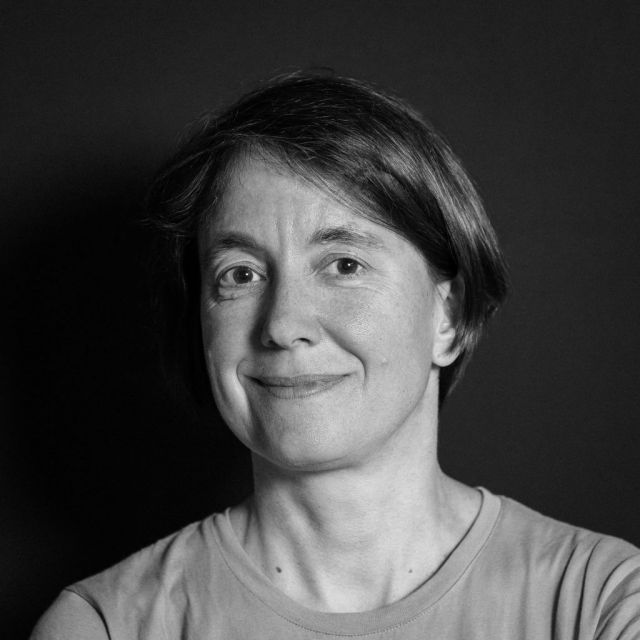
\includegraphics[width=0.5\textwidth]{kathrin.jpg} \\
}
\end{figure}

\noindent\textbf{Kathrin Passig} hat 27\% von \textit{Moby Dick} gelesen, weil das Buch zu lang ist. Sie hat schon mal eine Scheibe Wal gegessen, aber das war in Island und nur aus Höflichkeit.

\bigskip

\noindent\begin{minipage}{0.05\textwidth}
\vspace*{-5pt}
\reflectbox{
\includegraphics[width=16pt]{whale.png}}
\end{minipage}
\begin{minipage}{0.2\textwidth}
{@}kathrinpassig
\end{minipage}
\hspace{5pt}
\noindent\begin{minipage}{0.05\textwidth}
\vspace*{-5pt}
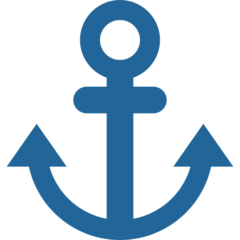
\includegraphics[width=16pt]{anchor.png}
\end{minipage}
\begin{minipage}{0.3\textwidth}
kathrin.passig.de
\end{minipage}

\bigskip

\begin{figure}[h]
{ \centering

\includegraphics[width=0.5\textwidth]{esther.jpg} \\
}
\end{figure}

\noindent\textbf{Esther Seyffarth} hat alle Stellen von \textit{Moby Dick} gelesen, in denen kein \textit{e} enthalten ist. Dann hat sie alle Stellen mit \textit{e} nachgeholt.

\bigskip

\noindent\begin{minipage}{0.05\textwidth}
\vspace*{-5pt}
\reflectbox{
\includegraphics[width=16pt]{whale.png}}
\end{minipage}
\begin{minipage}{0.12\textwidth}
{@}ojahnn
\end{minipage}
\hspace{5pt}
\noindent\begin{minipage}{0.05\textwidth}
\vspace*{-5pt}
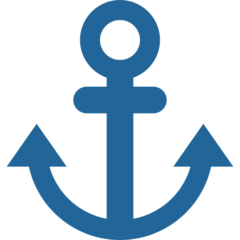
\includegraphics[width=16pt]{anchor.png}
\end{minipage}
\begin{minipage}{0.39\textwidth}
user.phil.hhu.de/\textasciitilde seyffarth
\end{minipage}
\noindent\begin{minipage}{0.05\textwidth}
\vspace*{-5pt}
\reflectbox{
\includegraphics[width=16pt]{elephant.png}}
\end{minipage}
\begin{minipage}{0.3\textwidth}
oulipo.social/{@}ojahnn
\end{minipage}

\end{document}
